% Section 8 (group C): Lambda and OP5, negative results
\section{\texorpdfstring{$\Lambda$}{Lambda} and OP5: negative results}
\label{sec:lop5}

This section reports what the construction does \emph{not} deliver for the cosmological constant.  The results are mostly negative: no
equation in the constructions of the Companion selects a value of $\Lambda$, the one dynamics that would produce the ratio $\Omega_M=\bsym^2$
either fails the data (H97) or puts that ratio in the future (H124), and the mediator that the local OP5 comparison model needs is causally
incompatible with the Higgs sector of the action W2.  The readout prediction H96 is open and will be decided by data.

\subsection{Two questions under one name}
\label{sec:lop5-split}

OP5 had two meanings in the Companion (\rnd{r05}, Decision~5.3).  In the architecture of the core it is the reversal-stable return readout of a
route whose source readout is OP1.  In physics it is the question of $\Lambda$, read in the core as a branching of a cascade,
$\Omega_\Lambda:\Omega_M=(1-\bsym^2):\bsym^2$, not as a dynamical vacuum energy (\cite{QSC}, \texttt{thm:dark-energy}).  On 6 November 2026 the
author separated three parts:
\begin{enumerate}
\item \emph{OP5 (core):} the reversal closure of the source--return pair.  It holds as a conditional schema under the assumptions of
\texttt{thm:op15-closure}; no native instance of the route with evaluable transports, class test and readout exists (\rnd{r11}, Theoremlet~11.2(a)).
\item \emph{$\Lambda$ readout:} whether $\Omega_\Lambda:\Omega_M=(1-\beta^2):\beta^2$ is the cascade branching, and at which epoch.  The epoch was fixed as
the present.
\item \emph{Action programme W1/W2:} a separate branch, frozen (Section~\ref{sec:act}).
\end{enumerate}
The historical chain that led from a spectral carrier through a trace formula to a bare $\Lambda$ term and a cancellation task lacks the step to a
well-defined metric action, and the size of the bare term does not follow.  The author suspended it as a foundation (\rnd{r11}, Decision~11.1).  The
working question since then is which independently defined quantity can be obtained by an explicit readout of the core, and which checkable
constraint follows.

Even the cascade only stabilises the ratio.  In the Markov cascade of the Companion the outflow fraction returns its input
$q=\lambda_-/\lambda_+=\tanh^2\eta$ for every rate; it does not derive it.  The register algebra admits a family of fields with any $0<q<1$ in the same
sector, so it does not select $q$ either (\rnd{r11}, Theoremlet~11.2(b),(c)).  The identification $q=\Omega_M(\text{today})$ is an additional assumption.

\subsection{H96 and H97}
\label{sec:lop5-h96}

Once the pair of counting rules is chosen, the $\Lambda$ readout gives a prediction without a free parameter (pre-registered; \rnd{r05}, Theoremlet~5.4):
\begin{equation}
 \Omega_M=\bsym^2=\frac{\gamma_L-1}{\gamma_L+1}=0.30185 .
 \label{eq:lop5-h96}
\end{equation}
It is decided by the first flat-$\Lambda$CDM value of $\Omega_m$ published after 6 November 2026 from DESI DR3 (BAO alone) or from Euclid,
confirmed within $2\sigma$.  The known values, DESI DR2 $0.2975\pm0.0086$ \cite{DESIDR2} ($0.5\sigma$) and Planck $0.3153\pm0.0073$
\cite{Planck2018}, are disclosed and do not count.  H96 rests on the U(1) counting per frame of Section~\ref{sec:beta} and on reading $\gamma_L$ as a
Lorentz factor.  Status \Open; no decisive data existed on 22 November 2026 (\rnd{r31}, Remark~31.6).

The only dynamics for the ratio in the Companion is the cascade with a return path.  A proposed bridge to cosmic time lets vacuum energy decay
into matter at the rate $\beta^2\Gamma$ with $\Gamma=\varepsilon H$.  With $\varepsilon=1$ it has no free parameter.  Test H97 (pre-registered,
not blind) compared it with the 13 DESI DR2 BAO values: $\chi^2_{\min}=105.0$ for 12 degrees of freedom, $p=6\times10^{-17}$.  H97 is
\Refuted.  The control, flat $\Lambda$CDM with free $\Omega_m$, reproduces DESI ($\Omega_m=0.2970$), and flat $\Lambda$CDM at $\Omega_M=\beta^2$ has
$\chi^2=10.9$, $p=0.54$ (\rnd{r05}, Theoremlet~5.5).

\subsection{The OP5 comparison model: a worked case}
\label{sec:lop5-worked}

The OP5 comparison model is a local auxiliary construction: a reduced field theory in which a matter modulation drives a comparison field whose
response can be read along a ray.  The worked case of \rnd{r32} collects its derivations; the algebraic steps (Theoremlets~32.2 and 32.4--32.6) were checked exactly in Wolfram Language.

\paragraph{What is chosen.}
Two inputs are set.  (i) The drive operator
\begin{equation}
 \mathcal P(\omega,\mathbf k)=\frac{\bigl[Z(\Omega_0^2+c_h^2q-x)+\tfrac32g_0^2d\bigr]d_m-g_m^2N_m}{m^2},
 \qquad N_m=\tfrac23\bigl(x^2-a_\perp x+a_\perp^2\bigr),
 \label{eq:lop5-drive}
\end{equation}
with $x=\omega^2$, $q=|\mathbf k|^2$, $a_\perp=|\mathbf k_\perp|^2$, $d=q-x$, $d_m=m^2+r_mq-x$.  It comes from a directed massive mediator of mass
$m$ plus the Einstein channel; the coefficients are chosen (one checked choice: $Z=1$, $r_m=c_h^2=\tfrac12$, $g_0^2=g_m^2=3/100$).
(ii) The identification of the radial Higgs source of matter with the drive of the comparison field, $\delta J_{\mathrm{OP5}}=\delta\mathcal J_h$.  It would
follow from a coupling $\int h\,\mathcal J_h$ in the same action that produces $\mathcal P$; no such action exists.

\paragraph{What follows.}
With the Higgs radius $h_{\mathrm W}=v+\eta_h$ of W2 and masses $m_i=y_ih_{\mathrm W}$, the radial source of non-relativistic matter is
$\mathcal J_h=-\sum_iy_in_i$, and a displacement $\mathbf u$ gives $\delta\mathcal J_h=(\sum_iy_in_{i0})\nabla\cdot\mathbf u$.  Two superposed elastic
continua with an internal spring can be prepared so that this source is switched on from rest while the energy--momentum tensor stays conserved
(Theoremlets~32.1, 32.2).

\begin{proposition}[compact ordinary response; \rnd{r32}, Theoremlet~32.3]
\label{prop:lop5-compact}
Let $V$ be smooth, spatially compact and zero before the switching, $D_0=\partial_t^2-\Delta$, and choose the preparation so that
$\delta\mathcal J_h=\mathcal P\,\delta H$ with $\delta H=-D_0\Delta^2V$.  Then $\delta T=-D_0T_*$ for a conserved tensor $T_*$ supported where $V$ is,
and in harmonic gauge with zero initial data and no incoming wave the linearised Einstein equation $D_0\bar\gamma_{\mu\nu}=16\pi G\,\delta T_{\mu\nu}$
has the solution $\bar\gamma_{\mu\nu}=-16\pi G\,T_{*,\mu\nu}$.  The ordinary linear curvature vanishes outside the support of $V$, also during
the switching.
\end{proposition}

\begin{proof}[Sketch]
$\delta T$ is linear in the preparation and the operators have constant coefficients, so $\delta T=-D_0T_*$.  Then $D_0(\bar\gamma+16\pi GT_*)=0$
with vanishing past data, whose retarded solution is zero.  Only linearity, constant coefficients and the initial data enter; the identification
(ii) does not.
\end{proof}

Under the identification (ii), the same source gives a non-zero directed contrast on the same axis: for a suitable compact profile with vanishing
transverse integral in every slice, the tidal readout of a ray along the axis is
$\Delta\mathcal I=16\mathcal AP/(m^2R^4)\neq0$, where $\mathcal A$ is the amplitude, $P$ the integrated longitudinal profile and $R$ the transverse
radius (Theoremlet~32.4).  The ordinary exterior is compact \Established; the contrast is \Conditional\ on (ii) and on the chosen
coefficients.  With a normalisation $\delta J_{\mathrm{OP5}}=c\,\delta\mathcal J_h$ the contrast scales with $c$, and whether $c\neq0$ is decided only
by a common action.  The case appears in shorter form in the v5.5.0 physics edition (development subsection ``A worked case'').

Figure~\ref{fig:lop5-slices} shows an earlier numerical object of the same comparison sector: one saved approximate field evaluated on six
coordinate-plane cuts.  It illustrates what the model provides at sampled points (invertible coframes, a nonzero residual) and what it does not
(an exact regional solution).

\begin{figure}[p]
\centering
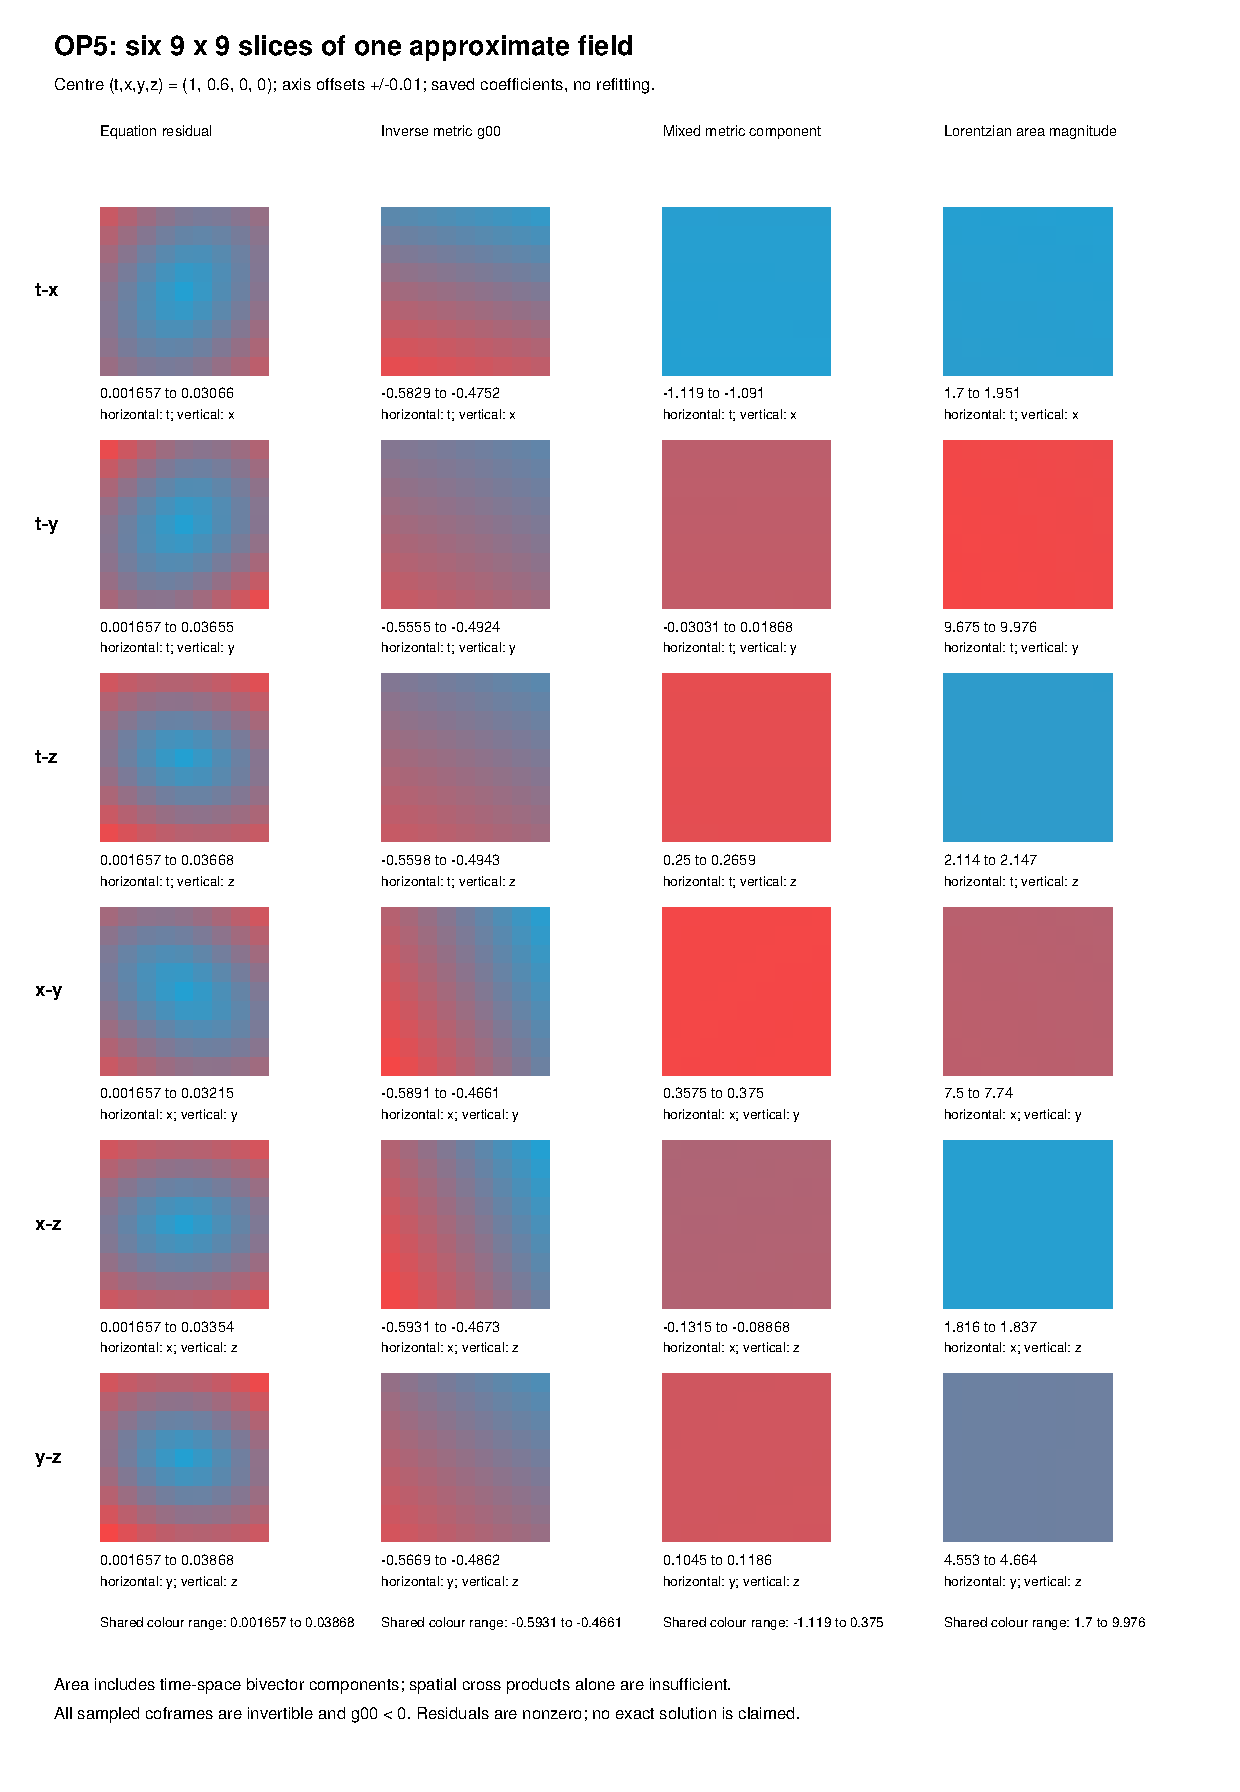
\includegraphics[width=\textwidth,height=0.66\textheight,keepaspectratio]{figures/F9-op5-slices.pdf}
\caption{OP5 comparison field, original affine baseline of 29 October 2026 (\cite{QSC}, subsection on the sampled multimode geometry; it predates
the worked case of \rnd{r32}).  Six overlapping $9\times9$ cuts through $(t,x,y,z)=(1,0.6,0,0)$ with offsets $\pm0.01$ of one saved approximate
field, a sum of two exponential modes, evaluated without refitting.  Columns: full probe-equation residual norm, $g^{00}$, normalised mixed
metric component $g_{ij}/\sqrt{|g_{ii}g_{jj}|}$, Lorentzian area magnitude $\sqrt{|g_{ii}g_{jj}-g_{ij}^2|}$; common colour range per column.
Largest sampled residual $\approx0.0387$, smallest $|\det|$ of the coframe $9.699$, every sampled $g^{00}<0$.  These are finite-sample diagnostics,
not uniform bounds.  Status: the residual is nonzero; no exact regional solution, native action or OP5 closure is claimed.}
\label{fig:lop5-slices}
\end{figure}

\subsection{The mediator line: a no-go}
\label{sec:lop5-mediator}

Rounds \rnd{r33} to \rnd{r52} searched for the mediator behind the directed term of~\eqref{eq:lop5-drive}.  We summarise the outcome.

\paragraph{The directed term needs a distinguished frame.}
W2 itself does not supply the comparison data: for the scalar channel it forces $c_h=1$ and $g_0=g_m=0$, and no subluminal directed massive
mediator exists in W1/W2 (\rnd{r33}, \rnd{r34}).  An audit (\rnd{r45}) traced the directed term to its origin: it is an ordinary Fierz--Pauli
exchange of a set, conserved, directed source $S^{\mu\nu}$, built from a coupling to the curvature component $R_{0i0j}$ transverse to an axis $n$
in a frame $u$.  Indeed $S_{\mu\nu}S^{\mu\nu}-\tfrac13(S^\mu{}_\mu)^2=N_m$, with $S_{\mu\nu}S^{\mu\nu}=a_\perp^2-2a_\perp x+2x^2$ and
$S^\mu{}_\mu=2x-a_\perp$.  Over r33--r44 the number of free choices stayed at one while each round moved it.  What remains set is the directed
coupling with frame $u$ and axis $n$, the slowed propagation $r_m$, and the values: all three are data of a distinguished frame.  This exposes a
fork: these data belong either to a field or medium (field side) or to the readout (observer frame, measuring axis).

\paragraph{The readout side carries the frame but not the slowing.}
Read as a readout, the directed coupling is a transverse tidal readout of a detector moving with $u$, and orientation and slowing drop out of the
leading static contrast (\rnd{r46}).  The branch predicts a dependence on the detector motion of relative size $v^2/c^2$ in the detector velocity $v$, very small at
laboratory velocities.  But the reduced model must also satisfy the metric cone limit, i.e.\ no characteristic propagates faster than the
metric light cone.  In the principal part of the model, $r_0$ and $r_m$ are the squared speeds of the massless and the massive mediator,
$\alpha=a_\perp/q\in[0,1]$, and the mediators couple to the Higgs radius with $j_0^2=\tfrac12g_0^2\alpha^2$ and
$j_m^2=\tfrac23g_m^2(r_m^2-r_m\alpha+\alpha^2)$.  With $Z=1$, $g_0^2=g_m^2=3/100$ the largest squared characteristic speed is $0.675$ for the chosen slow values, but $1.064$
for luminal mediators and $1.199$ with $c_h^2=1$ as W2 forces (\rnd{r47}, Theoremlet~47.1).  A Lorentz-covariant field propagates luminally in
every frame, so the slowing needs a distinguished frame on the field side.  The rest frame R of the field of Convention~F can slow propagation only
across its axis (\rnd{r49}, Theoremlets~49.1, 49.2).

\begin{proposition}[no-go for the luminal Higgs radius; \rnd{r49}, Theoremlet~49.3, found afterwards]
\label{prop:lop5-nogo}
For $c_h^2=1$ the left side of the upper condition of the cone limit of the reduced model, which has to be non-negative, is identically
\[
 -\tfrac23g_m^2(1+r_m-\alpha)-\frac{j_0^2}{1-r_0}-\frac{j_m^2}{1-r_m}<0
\]
for all mediator speeds $r_0,r_m\in(0,1)$, all $\alpha\in[0,1]$ and all $g_m>0$.  With the luminal Higgs radius of W2, the directed coupling
violates the metric cone limit for every choice of mediator.
\end{proposition}

\begin{proof}
All three terms are non-positive for $\alpha\le1<1+r_m$, and the first is strictly negative.  (The Companion checks the substitution with sympy.)
\end{proof}

The identification of the comparison field with the radial mode of W2 and the directed coupling are therefore causally incompatible for every
mediator, on either side of the fork \Refuted.  Three propagations would have to be slowed, and each needs a medium with its own rest vector.

\paragraph{A medium, and a vacuum bound.}
A medium of two light-like counter-streams (an object of the photon frame seen from other frames) can keep the cone limit for observers near the balance of the streams; one stream cannot
(H120, \rnd{r50}).  For any medium with a universal slowing $r=1-\epsilon$ in vacuum the upper cone condition gives (for $Z=1$, $g_0=g_m$) exactly
$\epsilon^2\ge g_m^2\bigl(\tfrac23-\tfrac23\alpha+\tfrac76\alpha^2\bigr)$, sharpest at $\alpha=1$, hence $\epsilon\ge\sqrt{7g_m^2/6}$.  Adopting the
laboratory bound $\epsilon\le10^{-13}$ on Lorentz violation (a bound for electrons \cite{Altschul2010}, used here for the Higgs sector without separate evidence) gives
\begin{equation}
 g_m^2\le\tfrac67\times10^{-26}\approx8.6\times10^{-27},
 \label{eq:lop5-bound}
\end{equation}
so the comparison model with $g_m^2=3/100$ is excluded in vacuum by about 25 orders of magnitude.  An observable directed contrast needs a
material whose rest frame is the preparation.  Reading the medium through the frame map $J_B$ instead does not carry: a medium that narrows the cone
in M widens it in T (cone value $0.803$ in M, $4.66$ for the $J_B$ image), so no medium keeps the limit in both (\rnd{r51}).

\subsection{\texorpdfstring{$\Lambda$}{Lambda} as an input}
\label{sec:lop5-input}

After this the author chose a negative closure of the OP5 remainder (\rnd{r56}; exploration, not blind).  Let $\mathcal K$ be the list of
constructions of the Companion that bear on a vacuum term: the frame maps as passive invertible maps and their dimensionless readouts; the reduced
actions of W1/W2; the semiclassical route from relative entropy; the OP5 comparison model; and the Markov cascade with its bridges to cosmic time.
$\mathcal K$ is a list of the record, not the class of all extensions.

\begin{proposition}[\rnd{r56}, Theoremlets~56.2--56.4]
\label{prop:lop5-input}
\textup{(a)} No construction in $\mathcal K$ has an equation that selects a value of the constant.  In W1/W2 the shift $V\to V+c$ of the potential
leaves the field equation unchanged and adds a $w=-1$ source.  Where the metric equations hold only in their trace-free part, the Bianchi identity and
$\nabla^aT_{ab}=0$ give $R+\kappa T=4\Lambda$ with $\Lambda$ an integration constant; in flat FLRW, $\dot H=-\tfrac\kappa2(\rho+p)$ and
$\dot\rho=-3H(\rho+p)$ imply $\tfrac{d}{dt}\bigl(H^2-\kappa\rho/3\bigr)=0$.
\textup{(b)} $\mathcal K$ fixes only dimensionless numbers of order one and contains no length of its own, whereas $\Lambda\ell_P^2=2.85\times10^{-122}$
(Planck 2018 input, $H_0=67.4$\,km\,s$^{-1}$Mpc$^{-1}$, $\Omega_\Lambda=0.6847$ \cite{Planck2018}).
\textup{(c)} With $\rho_M\propto a^{-3}$ and $\rho_\Lambda=\Lambda/\kappa$, the condition $\Omega_M(a)=\beta^2$ has for every $\Lambda>0$ exactly one
solution $a_*$, at which
\begin{equation}
 \Lambda=3(1-\beta^2)\,H_*^2=2.0944603\,H_*^2 .
 \label{eq:lop5-epoch}
\end{equation}
\end{proposition}

\begin{proof}
(a) $\tfrac{d}{dt}(H^2-\kappa\rho/3)=2H\dot H-\kappa\dot\rho/3=-\kappa H(\rho+p)+\kappa H(\rho+p)=0$.  (c) $\Omega_M$ decreases monotonically from
$1$ to $0$ as $a$ grows, so $\Omega_M=\beta^2$ has one solution; there $\rho_\Lambda=\rho_M(1-\beta^2)/\beta^2$ and
$H_*^2=\kappa(\rho_M+\rho_\Lambda)/3=\kappa\rho_\Lambda/\bigl(3(1-\beta^2)\bigr)=\Lambda/\bigl(3(1-\beta^2)\bigr)$.  The remaining statements are read from
the Companion and checked there in Wolfram Language.  (Round r56.4 wrote $\rho_\Lambda=3\Lambda/\kappa$, which does not fit relation~\eqref{eq:lop5-epoch}; the normalisation used here,
$\rho_\Lambda=\Lambda/\kappa$, is the one fixed in the correction \rnd{r61}, Theoremlet r61.1.)
\end{proof}

So the readout $\Omega_M=\beta^2$ holds at some epoch for every value of $\Lambda$; it fixes $\Lambda$ only in units of the Hubble rate at that
epoch.  Of the pair (value of $\Lambda$, epoch of the readout) exactly one datum is free, and the decision ``today'' supplies it.  Within $\mathcal K$
the absolute value of $\Lambda$ is an input, as in general relativity and unimodular gravity, and the coincidence ``why now'' is the same input, not
a second one \Established\ (for the list $\mathcal K$).  A construction outside $\mathcal K$ with its own length, or with a dimensionless number near
$10^{-122}$, would escape the statement.

\subsection{An attractor at \texorpdfstring{$\beta^2$}{beta squared} (H124)}
\label{sec:lop5-attractor}

The remaining route was a dynamics whose attractor is $\Omega_M=\beta^2$ (\rnd{r57}).

\begin{proposition}[\rnd{r57}, Theoremlet~57.1]
\label{prop:lop5-attractor}
Let vacuum energy decay into matter at rate $\delta H$ with $\delta=\varepsilon\beta^2$, in a flat universe without radiation:
$\rho_M'=-3\rho_M+\delta\rho_V$, $\rho_V'=-\delta\rho_V$, where $'=d/dN$, $N=\ln a$.  Then
\begin{equation}
 \frac{d\Omega_M}{dN}=(1-\Omega_M)(\varepsilon\beta^2-3\Omega_M).
 \label{eq:lop5-flow}
\end{equation}
The fixed points are $\Omega_M=1$ (repelling for $\varepsilon\beta^2<3$) and $\Omega_M^*=\varepsilon\beta^2/3$ (attracting).  Hence
$\Omega_M^*=\beta^2$ exactly for $\varepsilon=3$, one cascade step per e-fold of volume, with $w_{\mathrm{eff}}=-1+\beta^2=-0.698$ on the attractor.
\end{proposition}

\begin{proof}
With $\rho=\rho_M+\rho_V$ one has $\rho'=-3\rho_M$, so
$\Omega_M'=\rho_M'/\rho-\Omega_M\rho'/\rho=-3\Omega_M+\delta(1-\Omega_M)+3\Omega_M^2=(1-\Omega_M)(\delta-3\Omega_M)$.  The derivative of the right side is
$-\delta+6\Omega_M-3$ at $\Omega_M$; it is $3-\delta>0$ at $1$ and $\delta-3<0$ at $\delta/3$.  On the attractor $\rho'/\rho=-3\Omega_M^*=-3(1+w_{\mathrm{eff}})$.
\end{proof}

The value $\varepsilon=3$ follows from the demand ``attractor $=\beta^2$'', not from the structure.  The pre-registered, not blind test H124
compared the model with $\varepsilon=3$, radiation included and $\Omega_{M0}\in(\beta^2,1)$ and $hr_d$ free, with the 13 DESI DR2 BAO values;
refutation was set at $\chi^2_{\min}>24.72$ ($p<0.01$, 11 degrees of freedom).  Result: $\chi^2_{\min}=18.42$, $p=0.072$, at $\Omega_{M0}=0.5006$
and $hr_d=95.49$\,Mpc.  The model is not excluded by BAO alone, but it is worse than flat $\Lambda$CDM with the same number of free parameters by
$\Delta\chi^2=7.87$ (Figure~\ref{fig:lop5-attractor}).  The fit puts $\Omega_M$ today near $0.50$: the value $\beta^2$ lies in the future, so the
attractor does not explain ``why now'', and the epoch remains an input as in Proposition~\ref{prop:lop5-input}.  Explored afterwards: with
$\Omega_{M0}$ free, BAO allows small $\varepsilon$ as well as $\Lambda$CDM ($\varepsilon=1$: $\chi^2=9.35$), and $\chi^2$ rises only towards
$\varepsilon=3$.  CMB, supernovae and growth were not tested.

\begin{figure}[t]
\centering
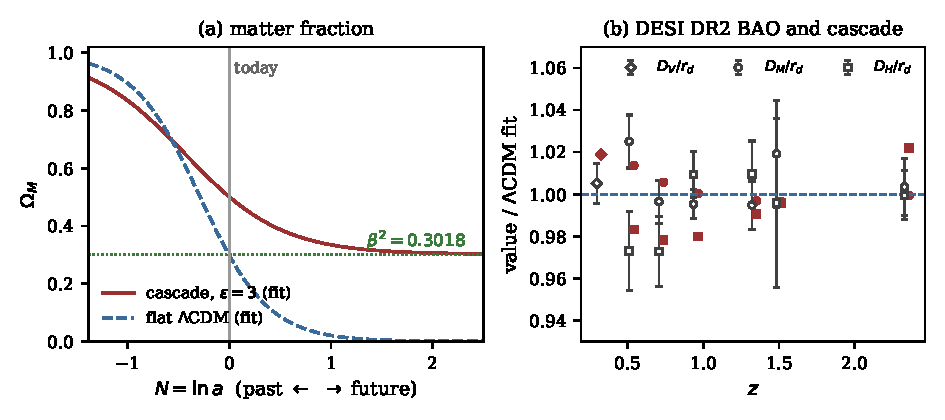
\includegraphics[width=\textwidth]{figures/F10-attractor.pdf}
\caption{Cascade with attractor $\Omega_M=\beta^2$ (H124).  (a) Matter fraction against $N=\ln a$ for the best-fitting cascade with
$\varepsilon=3$ ($\Omega_{M0}=0.5006$) and for flat $\Lambda$CDM ($\Omega_m=0.2970$), both fitted to DESI DR2 BAO \cite{DESIDR2}; the cascade
approaches $\beta^2=0.3018$ only in the future.  (b) The 13 BAO values (open symbols, $1\sigma$ diagonal errors) and the cascade prediction (filled,
slightly offset in $z$), each divided by the $\Lambda$CDM fit; each model has its own fitted $hr_d$.  Generated by
\texttt{scripts/F10\_attractor.py} from the data and model code of the H97/H124 tests in the Companion notes, which reproduces
$\chi^2_{\min}=18.42$ and $\Delta\chi^2=7.87$.  Status: H124 not excluded by BAO, not blind; the attractor does not fix the epoch.}
\label{fig:lop5-attractor}
\end{figure}

\subsection{Summary}
\label{sec:lop5-summary}

\begin{center}\small
\begin{tabular}{@{}p{0.48\textwidth}p{0.44\textwidth}@{}}
\toprule
statement & status\\
\midrule
H96: $\Omega_M=\bsym^2=0.30185$ today & \Open; decided by DESI DR3 or Euclid\\
H97: cascade bridge with $\varepsilon=1$ & \Refuted\ ($p=6\times10^{-17}$)\\
compact ordinary response of a prepared source & \Established\ (r32.3)\\
directed contrast on the same axis & \Conditional\ on a source identification without action\\
directed coupling with the luminal Higgs radius of W2 & \Refuted: violates the cone limit for every mediator\\
directed coupling in vacuum & $g_m^2\lesssim10^{-26}$ under the laboratory bound\\
$\Lambda$ within $\mathcal K$ & input; equivalent to the epoch of the readout\\
H124: attractor at $\varepsilon=3$ & not excluded by BAO ($p=0.072$), $\Omega_{M0}\approx0.50$, $\Delta\chi^2=7.87$\\
OP5 & \Open; core closure only as a conditional schema\\
\bottomrule
\end{tabular}
\end{center}
